\chapter{Network}

\section{Overview}
LON-CAPA has logical layers, see Fig.~\ref{fig:overview}:
\begin{itemize}
\item Clients to to particular servers in the network
\item Requests from clients are handled by handlers (at the ``ui'' level)
\item Handlers talk to the web service layer (the ``entity'' level) --- the webservices layer abstracts away the fact that the network is distributed
\item Databases and file systems
\end{itemize} 

\begin{figure}
\begin{center}
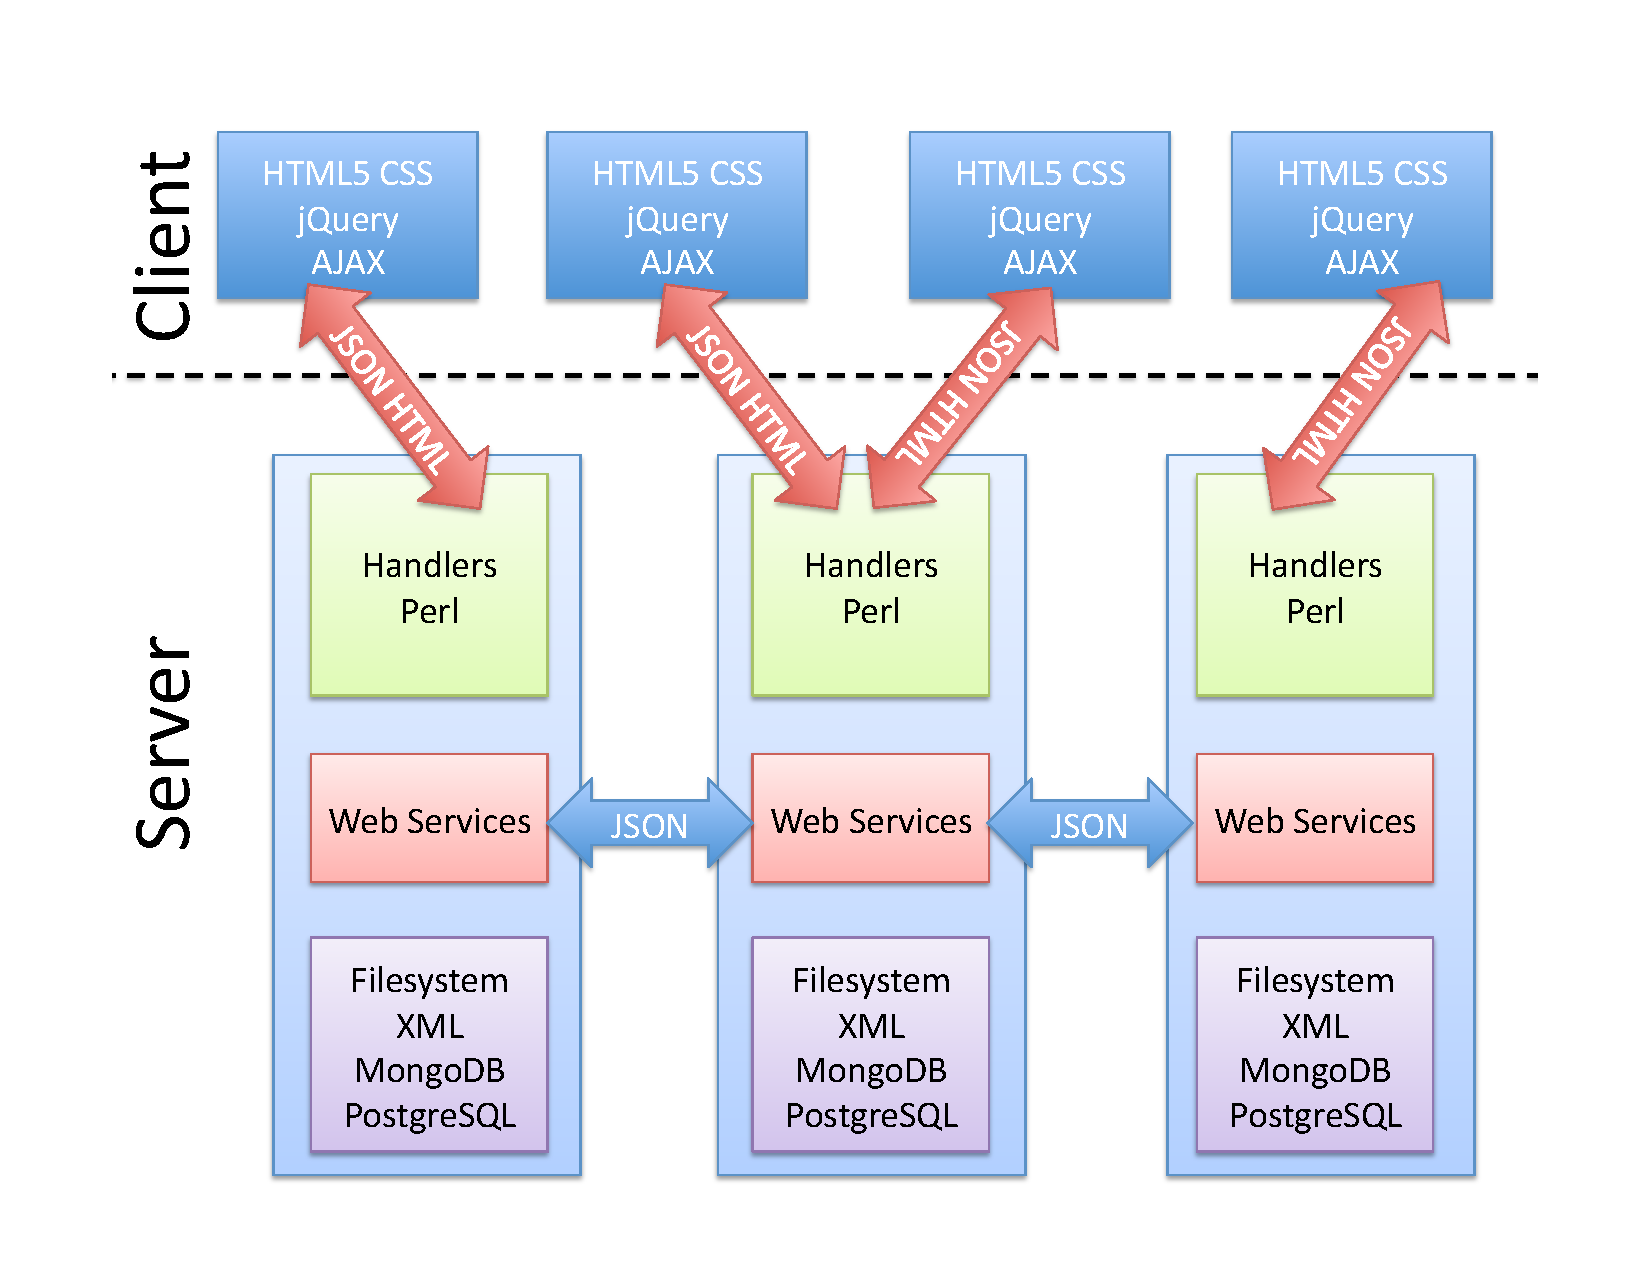
\includegraphics[width=12cm]{overview}
\end{center}
\caption{General overview of LON-CAPA Next Generation.\label{fig:overview}} 
\end{figure}

\section{Nodes}
LON-CAPA is built as a network of servers, which can host sessions and store data. LON-CAPA can have several independent clusters of such servers, but it is expected that in real operation, there is essentially one production cluster. In principle, any server in a cluster can host sessions for any user in the cluster, and any server in the network should be able serve any asset in the system. In practice, limitations may be put on this to preserve privacy and copyright.

\index{library server}\index{access server}
There are two classes of servers: access and library. The difference is that library servers permanently store data, and access servers do not. This means that library servers need to remain stable and have backup, which access servers can be added or removed on demand to absorb session loads.
\section{Cluster Table}
\subsection{Configuration}\index{cluster table}\label{clustertable}
Clusters are established by cluster tables, see below for an example
\begin{verbatim}
{ domains   : { 'msu'      :    { name    : 'Michigan State University',
                                  class   : 'university',
                                  locale  : 'en-us', 
                                  timezone: 'America/Detroit' },
                'sfu'      :    { name    : 'Simon Fraser University',
                                  class   : 'university',
                                  locale  : 'en-ca',
                                  timezone: 'America/Vancouver' },
                'ostfalia' :    { name    : 'Ostfalia University of Applied Sciences',
                                  class   : 'university',
                                  locale  : 'de',
                                  timezone: 'Europe/Berlin' },
                'elps'     :    { name    : 'East Lansing Public Schools',
                                  class   : 'k12',
                                  locale  : 'en-us',
                                  timezone: 'America/Detroit' }
              },
  hosts     : { 'zaphod'   :    { address : 'zaphod.localdomain',
                                  default : 'msu',
                                  domains : { 'msu'      : { function : 'library' },
                                              'elps'     : { function : 'library' },
                                              'sfu'      : { function : 'access'  }
                                            }
                                },
                'marvin'   :    { address : 'marvin.localdomain',
                                  default : 'msu',
                                  domains : { 'msu'      : { function : 'library' },
                                              'elps'     : { function : 'access'  },
                                              'sfu'      : { function : 'access'  }
                                            }
                                },
                'arthur'   :    { address : 'arthur.localdomain',
                                  default : 'sfu',
                                  domains : { 'msu'      : { function : 'access'  },
                                              'elps'     : { function : 'access'  },
                                              'sfu'      : { function : 'library' }
                                            }
                                },
                'slarti'   :    { address : 'slartibartfast.localdomain',
                                  default : 'ostfalia',
                                  domains : { 'ostfalia' : { function : 'library' },
                                              'elps'     : { function : 'access'  },
                                              'sfu'      : { function : 'access'  }
                                            }
                                }
              }
}
\end{verbatim}
Thus a particular server can serve more than one domain in different functions. Internally, servers are identified by the internal ID, e.g. ``slarti'' --- this allows migrating nodes between hardware.
\subsection{Homeservers}\index{homeserver}\label{homeserver}
Each entity in the system has a so-called homeserver within its domain which holds the authoritative and permanent copy of their data.
\subsection{Cluster manager}\index{cluster manager}
One server in any cluster is the cluster manager. This machine holds the authoritative copy of the cluster configuration table. 
Who is cluster manager is configured in
\begin{verbatim}
/home/loncapa/cluster/cluster_manager.conf
\end{verbatim}
This needs to be the full DNS name of the cluster manager, and essentially configures which cluster a server is a member of.

The cluster manager can trigger updating this table on other servers via
\begin{verbatim}
# On non-cluster manager, this triggers fetching the cluster table
#
<Location /fetch_cluster_table>
SetHandler perl-script
PerlHandler Apache::lc_init_cluster_table
SSLRequireSSL
SSLVerifyClient require
SSLVerifyDepth 2
</Location>
\end{verbatim}
The other server will then fetch the cluster table via the cluster manager's
\begin{verbatim}
# Cluster manager serves up authoritative cluster table
#
<Location /cluster_table>
SetHandler perl-script
PerlHandler Apache::lc_cluster_table
SSLRequireSSL
SSLVerifyClient require
SSLVerifyDepth 2
</Location>
\end{verbatim}
\section{Connections}
Connections between the servers are mediated via https.
\subsection{Connection authentication}\index{certificates}
Connections are authenticated via a configuration in lc.conf:
\begin{verbatim}
<Location /connection_handle>
SetHandler perl-script
PerlHandler Apache::lc_connection_handle
SSLRequireSSL
SSLVerifyClient require
SSLVerifyDepth 2
</Location>
\end{verbatim}
The certificates need to be located in /home/loncapa/certs/.

\subsection{Connection handling}
Connections are handled by the module lc\_connection\_handle. Any routines that should be externally accessible need to be registered with the module, like so:
\begin{verbatim}
BEGIN {
    &Apache::lc_connection_handle::register('modify_namespace',undef,undef,undef,
                                            \&local_modify_namespace,'entity','domain','name','data');
    &Apache::lc_connection_handle::register('dump_namespace',undef,undef,undef,
                                            \&local_json_dump_namespace,'entity','domain','name');
}
\end{verbatim}
The first argument is the command name, the following three arguments will be used for additional security, the next argument is the pointer to the subroutine that deals with this, and the remaining arguments are the named arguments of the function.
\subsection{Local versus remote}
Routines need to determine if the data is local or remote, depending on the homeserver of the entity, like so:
\begin{verbatim}
#
# Dump namespace from local data source
#
sub local_dump_namespace {
   return &Apache::lc_mongodb::dump_namespace(@_);
}

sub local_json_dump_namespace {
   return &Apache::lc_json_utils::perl_to_json(&local_dump_namespace(@_));
}

#
# Get the namespace from elsewhere
#
sub remote_dump_namespace {
   my ($host,$entity,$domain,$name)=@_;
   my ($code,$response)=&Apache::lc_dispatcher::command_dispatch($host,'dump_namespace',
                                 "{ entity : '$entity', domain : '$domain', name : '$name' }");
   if ($code eq HTTP_OK) {
      return &Apache::lc_json_utils::json_to_perl($response);
   } else {
      return undef;
   }
}


# Dump current namespace for an entity
# Call this one
#
sub dump_namespace {
   my ($entity,$domain,$name)=@_;
   if (&Apache::lc_entity_utils::we_are_homeserver($entity,$domain)) {
      return &local_dump_namespace($entity,$domain,$name);
   } else {
      return &remote_dump_namespace(
             &Apache::lc_entity_utils::homeserver($entity,$domain),$entity,$domain,$name);
   }
}
\end{verbatim}
The named arguments are sent as JSON.

Most routines that register services are in /entities --- other handlers should use the routines provided in the entity-handlers and {\it never} directly access the disk, the databases, or the network. The routines to be called are the ones without ``local'' or ``remote.''

\section{Replication}\index{replication}\label{replication}
Assets are replicated between servers. Any server in the network can serve any asset in the server under the same URL path. This is transparent, i.e., the same URL path can be requested from any server, regardless of whether or not that asset is already locally present. The server needs to locate the asset in the network and replicate it if needed.

Assets are versioned. Replication works by copying a certain version of an asset from its homeserver using
\begin{verbatim}
<LocationMatch "^/raw/">
SetHandler perl-script
PerlAccessHandler Apache::lc_raw_acc
SSLRequireSSL
SSLVerifyClient require
SSLVerifyDepth 2
</LocationMatch>
\end{verbatim}
This separate address (as opposed to the normal ``/res'' address) is important, since we need the raw XML, not a rendered version.

The system independently caches the most recent version of a resource. Once this cache expires, a server again asks the homeserver of the asset what the most recent version is via the ``current\_version'' command that is registered by lc\_entity\_urls. If this is not the version currently stored, a new version is fetched.
